% LaTeX Präsentationsvorlage (2013) der TU Graz, rev12, 2013/01/31
\documentclass{beamer}
% \documentclass[aspectratio=169]{beamer}
\usetheme{tugraz2013}

\usepackage[backend=biber,
style=alphabetic,
natbib=true,
]{biblatex}
\addbibresource{references-biblatex.bib}

\title[test]{\textbf{Dynamic Programming vs. Reinforcement Learning}}
\author{Noah Ruhmer}
\date{11. October 2022}

%%%%%%%%%%%%%%%%%%%%%%%%%%%%%%%%%%%%%%%%%%%%%%%%%%%%%%%%%%%%%%%%%%%%%%%%%%%%
\begin{document}
%%%%%%%%%%%%%%%%%%%%%%%%%%%%%%%%%%%%%%%%%%%%%%%%%%%%%%%%%%%%%%%%%%%%%%%%%%%%
\titleframe
\section{Introduction}

\begin{frame}
  \frametitle{Content}
  \tableofcontents%[hideallsubsections] 
  \note{
  	
  }
\end{frame}

\begin{frame}
	\frametitle{Motivation}
	\begin{itemize}
		\item Learn theory of optimal control problems
		\item Compare between model-free and model-based approaches
		\item Apply dynamic programming and reinforcement learning in practice
		\item Compare these different methods
	\end{itemize}
	
\end{frame}

\section{Theory}
\begin{frame}
	\frametitle{Markov Decision Process}
	Describes a discrete-time dynamic process \cite{bellman1957markovian}. Useful for solving optimization problems via dynamic programming.
	\begin{itemize}
		\item States
		\item Actions
		\item Transitions (probabilistic)
		\item Cost/Reward
	\end{itemize}
	\textbf{Markov Property:}\\
	\textit{''Given the present, the future does not depend upon the past.''}
\end{frame}

\begin{frame}
	\frametitle{Dynamic Programming}
	Model-based mathematical optimization of a MDP \cite{bellman1966dynamic}. Sub-problems solved recursively retrieving an optimal policy.
	
	\begin{itemize}
		\item Requires optimal substructure (e.g. Shortest Path)
		\item Requires overlapping sub problems (e.g. Fibonacci)
	\end{itemize}
	\textbf{Stochastic Bellman Equation:}
	\begin{equation*}
	\label{eqn:sto_bellman}
	V(s) = \max_a \bigg(R(a, s) + \sum_{s'} P(a, s, s') V(s')\bigg)
	\end{equation*}

\end{frame}

\begin{frame}
	\frametitle{Reinforcement Learning}
	Trial and Error (Explorative) approach to estimate optimal policy.
	\note{Important to distinguish that it does reward outcome not actions}
	\begin{enumerate}	
		\item Observe state
		\item Choose action depending on state by using the policy
		\item Execute action
		\item Reward or punishment from environment
		\item Record information about reward for action-state pair
	\end{enumerate}
	\begin{itemize}
		\item Reward depending on outcome not actions
		\item Policy maximizes received reward
	\end{itemize}
\end{frame}

\begin{frame}
	\frametitle{Q-Learning}
	Model-free reinforcement learning algorithm \cite{watkins1989learning}. It does not need transition rules to learn.

	\begin{itemize}
		\item Uses table assigning each action-state pair a value
		\item Learning by exploration in the environment
		\item Policy is to pick action with highest Q-Value
		\item Converges to optimal policy \cite{watkins1992q}
	\end{itemize}
	
	\textbf{Q-Table update:}
	\begin{equation*}
		Q_{new}(a, s) = Q(a, s) + \alpha \cdot \bigg(R(a, s) + \gamma \cdot \max_a Q(a, s') - Q(a, s)\bigg)
	\end{equation*}
\end{frame}

\section{Example}
\begin{frame}
	\frametitle{Parking Problem}
	$N$ sequentially placed spaces where a driver wants to park with minimal cost. The driver is incrementally visiting the spaces observing only the current space \cite{bertsekas2019reinforcement}. 
	\begin{itemize}
		\item Place is free with probability $p$
		\item The last space N (garage) has a fixed cost $C$ and is free
		\item $c(i)$ decreasing from $N$ to $0$
	\end{itemize}
	There cost come only from transitioning to the parked state.
	Intuitive solution is to park as late as possible.
\end{frame}

\begin{frame}
	\frametitle{Parking Problem}
	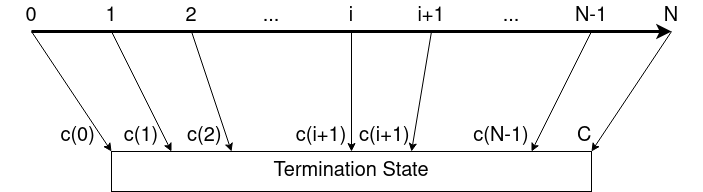
\includegraphics[width=1\textwidth]{figures/parking_graphic.png}\\
	\begin{itemize}
		\item $2 N$ states
		\item $2$ actions
	\end{itemize}
	Previous states do not influence the current. 
	Best policy to park after a threshold.
\end{frame}

\begin{frame}
	\frametitle{Dynamic Programming Solution}
	\vspace{-0.3cm}	
	\textbf{Recursive Value Function:}
	\begin{equation*}
		\begin{split}
			&V(i) = p \cdot c(i) + (1-p) \cdot V(i+1)\\
			&V(N) = C, \quad \forall i \colon0 \leq i < N
		\end{split}
	\end{equation*}
	
	\textbf{Explicit Value Function:}
	\vspace{-0.3cm}
	\begin{equation*}
		\begin{split}
			&V(i) = C \cdot (1-p)^{N-i} + \sum_{j=0}^{N-i} p \cdot (N-i-j) \cdot (1-p)^{j}
		\end{split}
	\end{equation*}
	\textbf{Optimal Expected cost:} $\max_i V(i) = V^* $
	\vspace{0.3cm}
	
	Parking at the first free space after this is optimal.
\end{frame}

\begin{frame}
	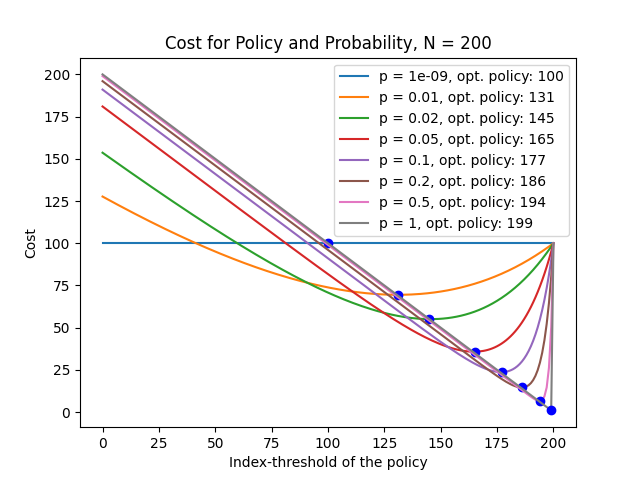
\includegraphics[width=0.9\textwidth]{figures/strategy_probabilities_200.png}
\end{frame}

\begin{frame}
	\frametitle{Q-Learning Rewards}
	\vspace{-0.3cm}
	Approximate the Dynamic Programming solution.
	
	\vspace{0.3cm}
	We want minimal cost, however Q-Learning uses maximal rewards.
	\vspace{0.3cm}
	
	\textbf{Total rewards:}
	\begin{itemize}
		\item Negate cost function
		\item Shift it to use only positive values
	\end{itemize}
	\textbf{Incremental rewards:}
	\begin{itemize}
		\item reward driving instead of parking
		\item sum of reward needs to be equal to other reward functions $\rightarrow$ negative reward in garage
	\end{itemize}
\end{frame}

\begin{frame}
	\frametitle{Q-Learning Training}
	\vspace{-0.3cm}
	Q-Table initialized to $0$.
	\vspace{0.3cm}
	
	\textbf{Parameters:}
	\begin{itemize}
		\item learning rate: $\alpha = 0.05$ and descending, higher for $N$ larger than $500$
		\item exploration rate: $\epsilon = 0.05$ and descending 
		\item discount factor: $\gamma = 0.999$ 
	\end{itemize}
	Results can be further improved by tuning these parameters and by increasing the training time.
\end{frame}

\begin{frame}
	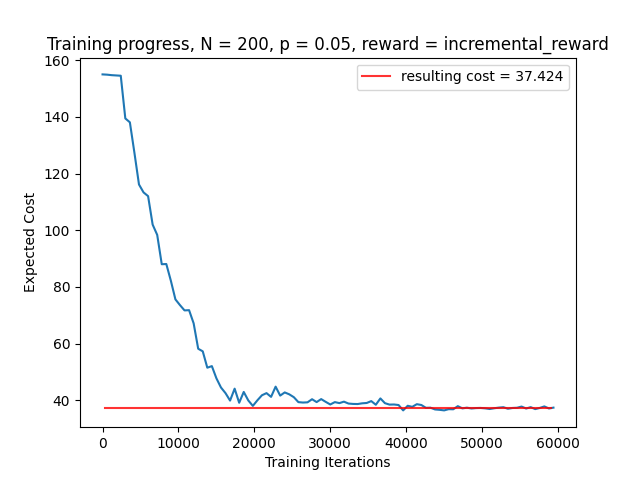
\includegraphics[width=0.9\textwidth]{figures/q_training_progress_200.png}
\end{frame}

\section{Results}

\begin{frame}
	\frametitle{Result Comparison}
	\centering
	\begin{tabular}{ |c|c|c|c| } 
		\hline
		N& \multicolumn{2}{c|}{Q-learning} & Dynamic Programming\\ 
		\hline
		-& $\mu$ & $\sigma$ & -\\ 
		\hline
		$50$ & $17.005$ & $0.263$ & $16.366$ \\ 
		\hline
		$100$ & $26.251$ & $0.519$ & $25.140$ \\ 
		\hline
		$200$ & $37.145$ & $0.989$ & $35.764$ \\ 
		\hline
		$500$ & $53.973$ & $1.591$ & $51.663$ \\ 
		\hline	
	\end{tabular}
	
	\vspace{0.5cm}
	\small Statistics from 20 independently learned policies
\end{frame}

\begin{frame}
	\frametitle{Conclusion}
	\vspace{-0.3cm}
	\textbf{Dynamic Programming}
	\begin{itemize}
		\item Full system model needed
		\item High requisites on the system
		\item Delivers an exact solution
	\end{itemize}
	\textbf{Reinforcement Learning}
	\begin{itemize}
		\item No system model needed
		\item Approximated solution
		\item Adaptive to similar problems
	\end{itemize}
	
	
	
\end{frame}

\section{Bibliography}
\begin{frame}
	\printbibliography
\end{frame}

%%%%%%%%%%%%%%%%%%%%%%%%%%%%%%%%%%%%%%%%%%%%%%%%%%%%%%%%%%%%%%%%%%%%%%%%%%%%
\end{document}
%%%%%%%%%%%%%%%%%%%%%%%%%%%%%%%%%%%%%%%%%%%%%%%%%%%%%%%%%%%%%%%%%%%%%%%%%%%%

%% EOF
